\section{方法}
\subsection{问题定义与框架概览} \label{subsec:overview}
\begin{figure*}[t]
    \centering
    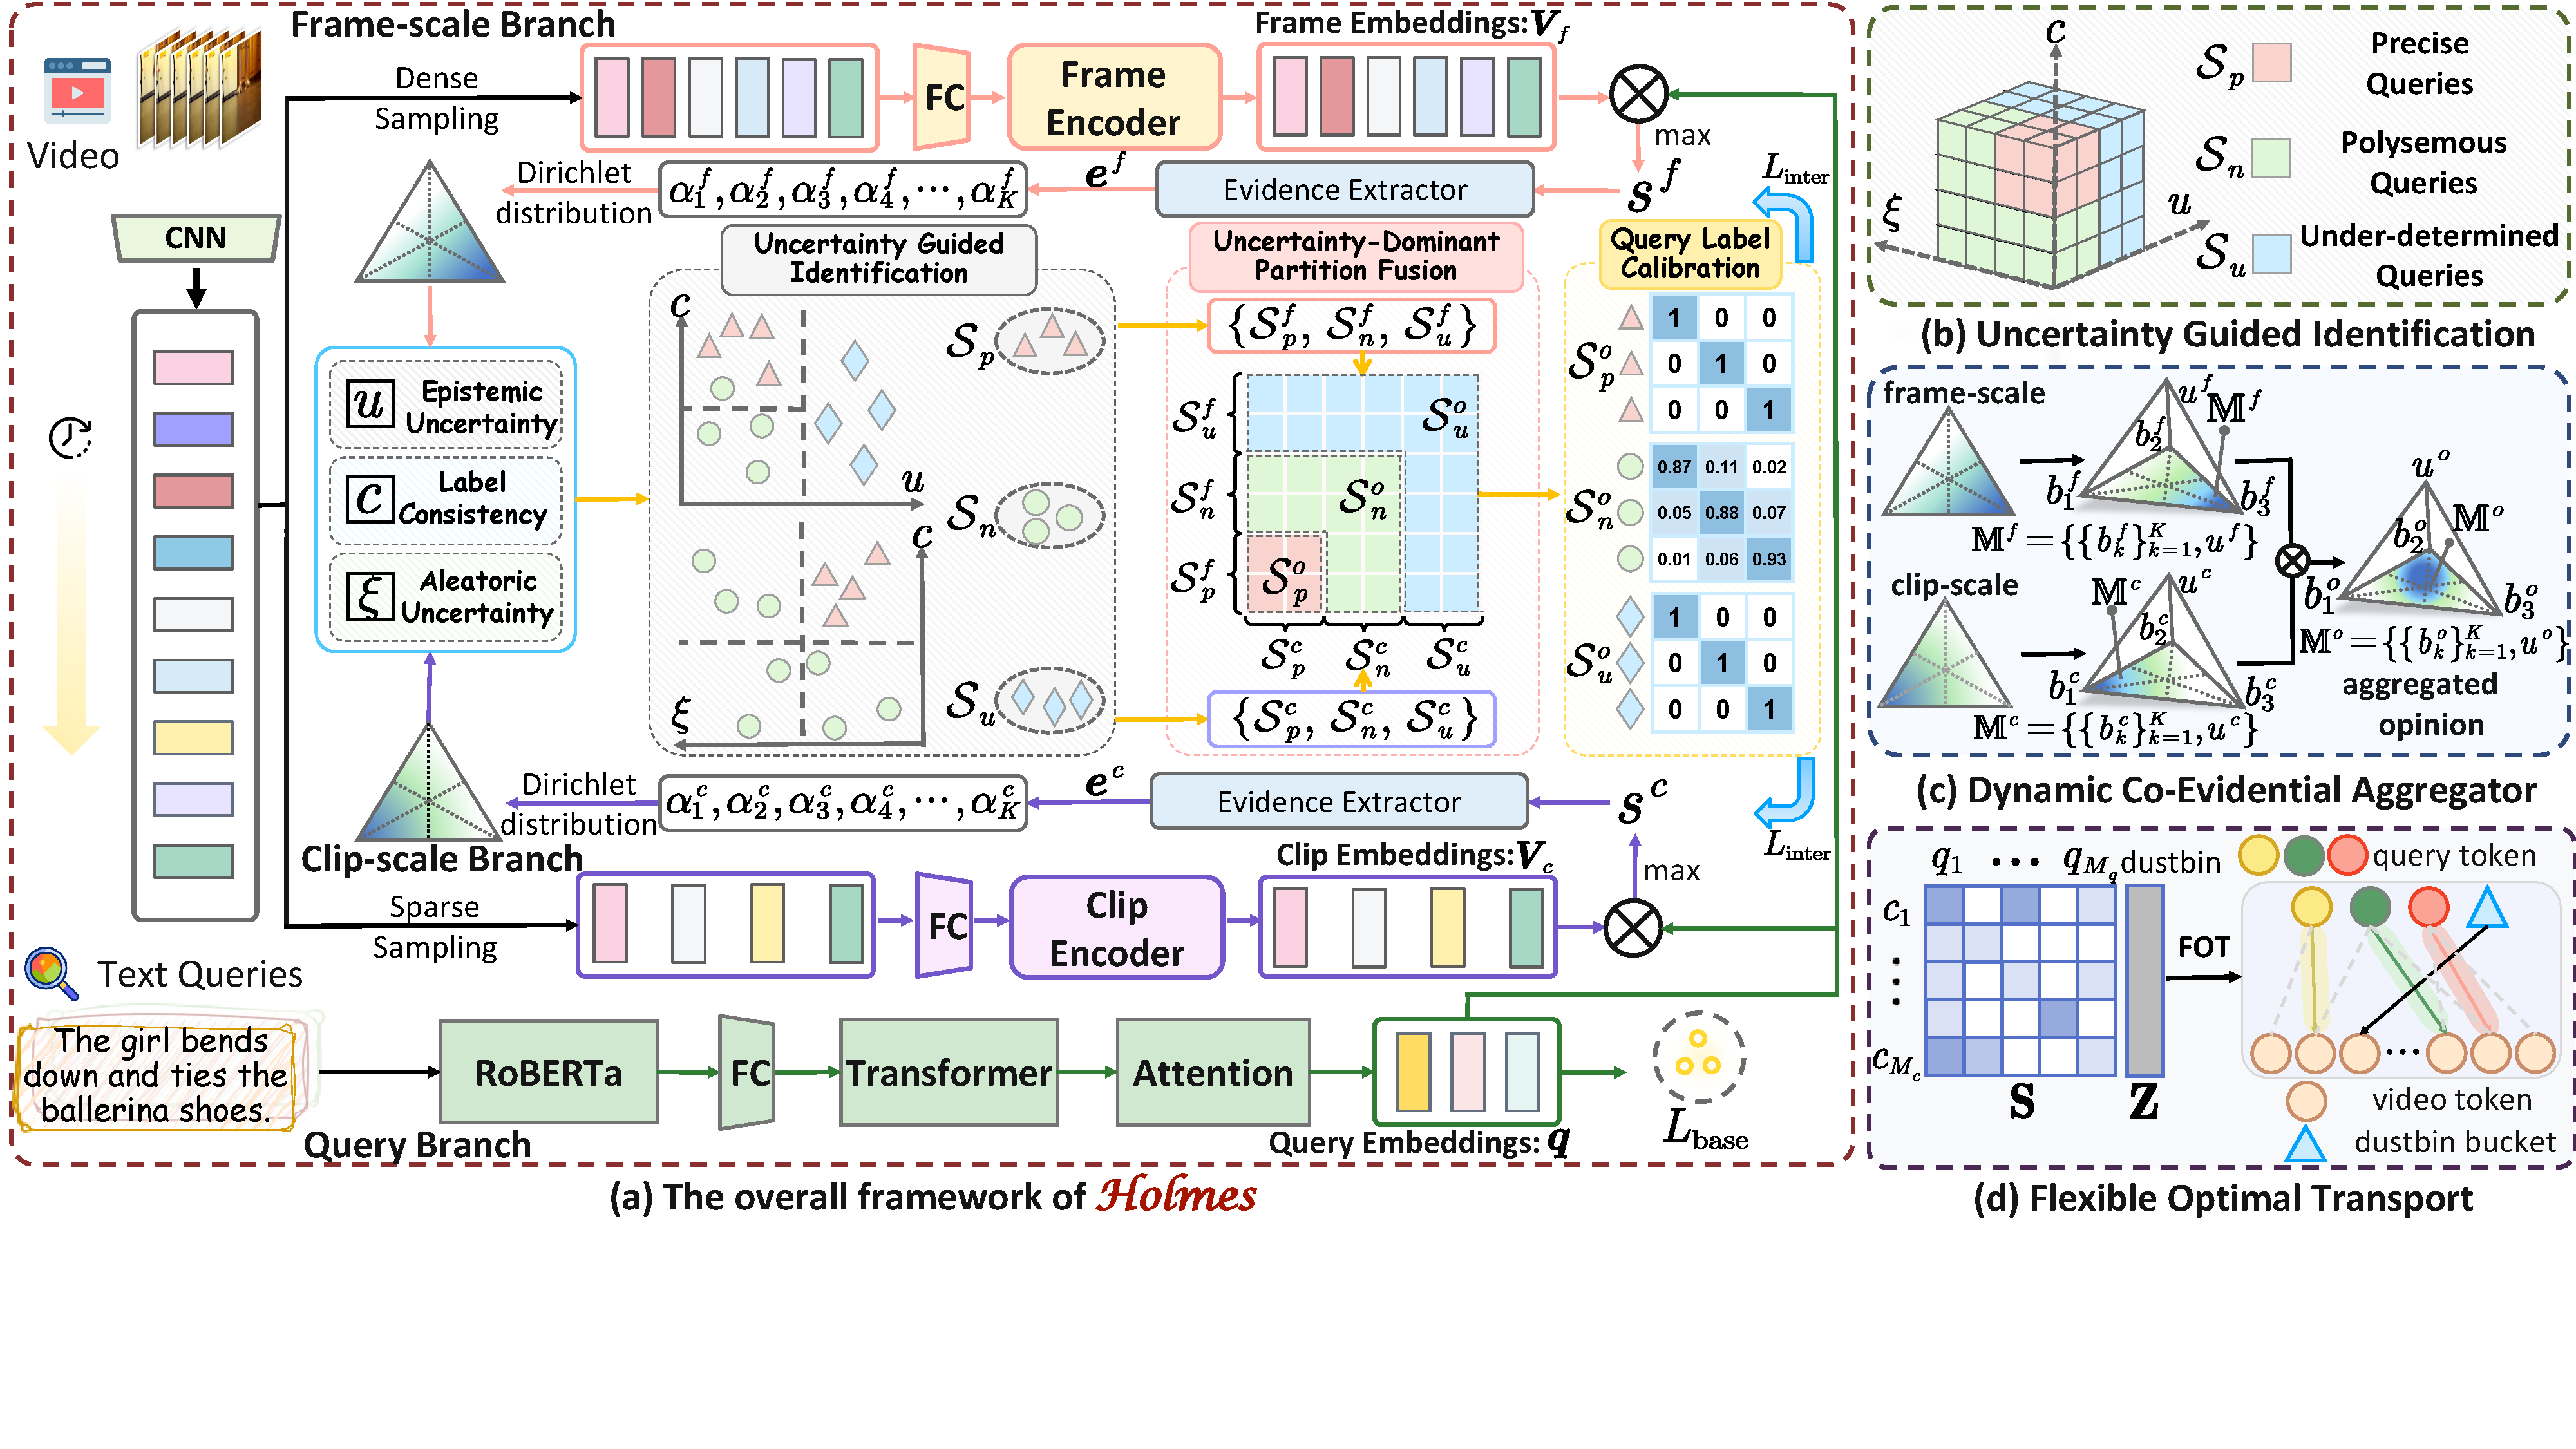
\includegraphics[width=\textwidth]{images/methodv3.pdf}
    \caption{\modelname{} 框架概览。
\textbf{(a)} 查询分支生成查询嵌入 $\bmq$，帧与片段尺度分支分别提取视频表征 $\bmV_f$ 和 $\bmV_c$，得到相似度分数 $S_f$ 和 $S_c$。将候选相似度转换为证据向量，以 Dirichlet 分布建模并估计三项判别量。不确定性引导识别据此将各尺度查询划分为精确查询（$\mathcal{S}^f_p$、$\mathcal{S}^c_p$）、多义查询（$\mathcal{S}^f_n$、$\mathcal{S}^c_n$）和信息不足查询（$\mathcal{S}^f_u$、$\mathcal{S}^c_u$）。不确定性主导的划分融合整合两种尺度的划分，得到 $\mathcal{S}^o_p$、$\mathcal{S}^o_n$ 和 $\mathcal{S}^o_u$。完成查询自适应的标签校准后，以修正后的标签通过 $L_{\mathrm{inter}}$ 监督视频间证据学习。
\textbf{(b)} 不确定性引导识别在三维潜在空间中划分查询，先在 $c$--$u$ 平面上粗分，再沿 $\xi$ 轴细分。
\textbf{(c)} 动态协同证据聚合器无需额外参数，即可融合两种尺度的证据意见。
\textbf{(d)} 灵活最优传输使用\emph{回收槽}吸收噪声片段，将可靠的查询与片段软分配作为视频内证据学习的标签证据。
    }
    \label{fig:arc}
\end{figure*}
部分相关视频检索旨在找出包含给定文本查询所描述时刻的视频。每个视频包含多个候选时刻，而每条查询对应相关视频中的某个特定时刻。本文提出分层证据学习框架 \modelname{}，从视频间和视频内两个层面处理 PRVR 的查询歧义，如\cref{fig:Intro}(a) 所示。下面先介绍三个组成部分。

\noindent \textbf{文本查询表征} \quad
先使用预训练的 RoBERTa~\cite{liu2019roberta} 对文本查询编码，再通过投影层和 Transformer~\cite{vaswani2017attention} 获取上下文化表征。与 MS-SL\cite{ms-sl} 类似，最终将表征聚合成 $\bmq \in \mathbb{R}^d$。

\noindent \textbf{视频表征} \quad 对于未经裁剪的视频，先用预训练 CNN 提取特征。参照已有工作\cite{GMMFORMER}，我们采用双分支架构提取多尺度表征。
帧尺度分支通过全连接层将采样所得的 $M_f$ 帧投影到 $d$ 维空间，再由帧编码器得到 $\bm{V_f} = \{\bmf_i\}_{i=1}^{M_f} \in \mathbb{R}^{M_f \times d}$。
片段尺度分支将视频稀疏划分成 $M_c$ 个片段，投影后送入片段编码器，得到 $\bm{V_c} = \{\bmc_i\}_{i=1}^{M_c} \in \mathbb{R}^{M_c \times d}$。

\noindent \textbf{相似度计算} \quad
为计算文本与视频配对 $(T, V)$ 的相似度，先获得 $\bmq$、$\bm{V_f}$ 和 $\bm{V_c}$，再计算帧尺度与片段尺度的相似度分数：
\vspace{-.6em}
\begin{equation}
\begin{aligned}
s^f(T, V) = \text{max} \{ \text{cos}(\bmq, \bmf_1),..., \text{cos}(\bmq, \bmf_{M_f})\}, \\
s^c(T, V) = \text{max} \{\text{cos}(\bmq, \bmc_1),..., \text{cos}(\bmq, \bmc_{M_c})\}.
\label{eq:simscore}
\end{aligned}
\vspace{-.6em}
\end{equation}
随后计算文本与视频之间的总体相似度分数：
\vspace{-.6em}
\begin{equation}\label{eq:sim}
s({T}, {V}) = \alpha_f s^f({T}, {V}) + \alpha_c s^c({T}, {V}),
\vspace{-.6em}
\end{equation}
其中 $\alpha_f, \alpha_c \in [0,1]$，且 $\alpha_f + \alpha_c = 1$。最终按\cref{eq:sim} 给出的分数检索并排序视频。

\subsection{视频间证据学习}
本节通过视频间证据学习估计查询的不确定性，以此对查询歧义建模。我们先介绍查询识别的三项判别原则（\cref{fig:arc}(a)）。两个分支流程相似，以下以帧尺度分支为例。

\noindent \textbf{三项判别原则} \quad
对于查询 $\bmq_i$ 和 $K$ 个视频，先计算查询与第 $j$ 个视频的帧尺度相似度 $s^f_{ij}$（\cref{eq:simscore}），简记为 $s_{ij}$。
% Viewing retrieval as $K$-class classification,
沿用\citep{edl-2018} 的做法，从相似度导出证据：
\vspace{-.8em}
\begin{equation}
    e_{ij} = \exp\left(\tanh\left(s_{ij}/ \tau\right)\right), \quad 
    \boldsymbol{e}_i = [e_{i1}, \dots, e_{iK}],
    \vspace{-.8em}
    \label{ea:evi1}
\end{equation}
默认设 $\tau=0.1$。根据 Dempster-Shafer 理论（DST）\cite{dst}，可利用证据量化认知不确定性，反映数据对查询与候选视频关联的支持程度。
% Following Subjective Logic (SL) \cite{ edl-2018}, 
首先将证据 $ {e}_i$ 映射为 Dirichlet 分布参数：
\vspace{-.8em}
\begin{equation}
    {\boldsymbol \alpha}_i = [\alpha_{i1}, \dots, \alpha_{iK}], \quad \alpha_{ij} = e_{ij}+1.
    \label{eq:dir-alpha}
    \vspace{-.6em}
\end{equation}
\begin{definition}\textbf{认知不确定性。} 对于查询 $\bmq_i$，认知不确定性 $u_i$ 和信念质量 $b_{ij}$ 定义为
\vspace{-1.em}
\begin{equation}
    u_i = \frac{K}{S_i}, \quad b_{ij} = \frac{\alpha_{ij}-1}{S_i}, \quad 
    S_i = \sum_{j=1}^{K} \alpha_{ij},
    \label{eq:dir-alpha2}
\vspace{-1.em}
\end{equation}
且 $u_i + \sum_{j} b_{ij} = 1$。这里，$S_i$ 表示 Dirichlet 分布的强度，$ {\boldsymbol b}_i = [b_{i1}, \dots, b_{iK}]$ 表示由 $ {\boldsymbol \alpha}_i$ 导出的主观意见。
\vspace{-.8em}
\end{definition}
较高的 $u_i$ 反映证据有限、模型对查询理解不足，可用于识别信息不足查询。但 $u_i$ 较低并不能保证检索精确。形式化地说：
\vspace{-.6em}
\begin{theorem}
较低的认知不确定性 $u_i$ 并不意味着最高信念一定分配给标注标签 $ {y}_{i}$。
\vspace{-.8em}
\begin{equation}
    \boldsymbol q_i \text{ 的 } u_i \text{ 较低} \nRightarrow \arg\max\, \boldsymbol{b}_{i} = \arg\max \boldsymbol{y}_{i}.
\vspace{-.8em}
\end{equation}
\label{theorem: wrong uncertainty}
\end{theorem}
\vspace{-2em}
证明见附录 \ref{appendix:theorem3.2}。$\boldsymbol{y}_i = [y_{i1}, \dots, y_{iK}]$ 是独热真实标签。该定理表明，仅凭认知不确定性无法保证信念集中在标注视频上，因此我们引入标签一致性原则。
\begin{definition} \textbf{标签一致性。} 对于查询 $\bmq_i$，标签一致性 $c_i$ 定义为：
\vspace{-.6em}
    \begin{equation}
        c_{i}=\max (0, \boldsymbol{s}_{i}\cdot \boldsymbol{y}_{i}),
        \label{eq: cons}
\vspace{-.6em}
    \end{equation}
其中 $\boldsymbol{s}_i = [s_{i1}, \dots, s_{iK}]$ 表示相似度分数。
\vspace{-.6em}
\end{definition}
较低的 $c_i$ 表明查询与真实匹配视频的对齐较差，但较高的 $c_i$ 并不能说明查询精确。形式化地说：
\begin{proposition}
较高的标签一致性 $c_i$ 并不意味着该查询是精确查询。
\vspace{-.6em}
\begin{equation}
    \boldsymbol q_i \text{ 的 } c_i \text{ 较高} \nRightarrow \boldsymbol q_i \text{ 是精确查询}.
    \vspace{-.8em}
\end{equation}
\label{theorem:wrong-consistency}
\vspace{-2em}
\end{proposition}
\vspace{-.6em}
\begin{proof} 如\cref{fig:Intro}(c) 所示，真实匹配视频的响应较高并不意味着匹配精确，因为其他视频也可能具有同样高的相似度。
\vspace{-1em}
\end{proof}
为区分精确查询和多义查询，我们引入偶然不确定性\cite{au}，用\cref{eq:aleatoric-uncertainty} 中 $\text{Dir}({\boldsymbol\alpha_i})$ 下的期望熵来衡量。低熵表示概率质量集中于单个视频，表明查询可能是精确的。高熵则表示概率分布较为均匀，表明查询可能存在多义性。

\begin{definition} \textbf{偶然不确定性。}
对于查询 $\bmq_i$，偶然不确定性 $\xi_i$ 定义为
\vspace{-.6em}
\begin{equation}
\!\!\!\!\mathbb{E}_{\mathbf{p} \sim \text{Dir}({\boldsymbol\alpha_i})} [H(\mathbf{p})]\!\!=\!\!\sum_{k=1}^K \frac{\alpha_{ik}}{S_{i}} \left( \psi(S_{i} \!+ \!1) \!-\! \psi(\alpha_{ik}\! + \!1) \right),
\vspace{-.6em}
\label{eq:aleatoric-uncertainty}
\end{equation}
其中 $\psi$ 表示 digamma 函数，定义为 $\psi(x) = \frac{d}{d x} \log \Gamma(x)$，$H$ 表示 Shannon 熵。完整推导见附录 \ref{appendix:aleatoric-uncertainty}。
\vspace{-.6em}
\end{definition}

\noindent \textbf{不确定性引导识别} \quad \label{method:ugi}
依据上述原则，可将查询分为三类：
(i) 认知不确定性较高的信息不足查询 $\mathcal{S}_{u}$；
(ii) 认知不确定性较低、标签一致性较高的初步精确查询 $\mathcal{\tilde{S}}_{p}$；
(iii) 认知不确定性较低、标签一致性较低的初步多义查询 $\mathcal{\tilde{S}}_{n}$。
形式化表示如下：
\vspace{-.6em}
\begin{equation}
\begin{cases} 
\mathcal{S}_{u} = \{q_i \mid u_i > \beta_u\}, \\ 
\mathcal{\tilde{S}}_{p} = \{q_i \mid u_i \le \beta_u,\, c_i \ge \beta_p\}, \\
\mathcal{\tilde{S}}_{n} = \{q_i \mid u_i \le \beta_u,\, c_i < \beta_p\}.
\end{cases}    
\label{eq:initial-division}
\vspace{-.6em}
\end{equation}
阈值 $\beta_u$ 和 $\beta_p$ 按以下方式自适应确定：
\vspace{-.6em}
\begin{equation}
    \beta_u = \min(u^{tp}, 1 - \beta), \quad 
    \beta_p = \max(\beta, c^{tp}),
    \label{eq:threshold}
\vspace{-.6em}
\end{equation}
其中 $u^{tp}$=$\max_{i \in \mathcal{S}^{tp}} u_i$，$c^{tp}$ = $\min_{i \in \mathcal{S}^{tp}} c_i$，且 $\beta=0.3$。$\mathcal{S}^{tp}= \left\{ i \,\middle|\, \arg\max(\boldsymbol{s}_i) = \arg\max(\boldsymbol{y}_i) \right\}$ 表示正确匹配的查询与视频配对。在噪声对应学习中，$\mathcal{\tilde{S}}_{n}$ 通常被视为噪声配对，我们则将其解释为查询歧义的表现。含糊的语义可能削弱真实匹配视频的响应。命题 \ref{theorem:wrong-consistency} 表明，$\mathcal{\tilde{S}}_{p}$ 中也仍包含多义查询。进一步比较 $\xi$，对 $\mathcal{\tilde{S}}_{p}$ 细分，得到最终的精确查询集合 $\mathcal{S}_{p}$ 和多义查询集合 $\mathcal{S}_{n}$：
\vspace{-.6em}
\begin{equation}
\begin{cases}
\mathcal{S}_p = \{ q_i \in \mathcal{\tilde{S}}_p \mid \xi_i < \text{median}(\{\xi_j\}_{q_j \in \mathcal{\tilde{S}}_p}) \}, \\
\mathcal{S}_n = \bigl( \mathcal{\tilde{S}}_p \cup \mathcal{\tilde{S}}_n \bigr) \setminus \mathcal{S}_p.
\end{cases}
\label{eq:refined_partition}
\vspace{-.6em}
\end{equation}
\noindent\textbf{不确定性主导的划分融合} \quad
根据\cref{eq:initial-division,eq:refined_partition}，帧尺度与片段尺度分支分别生成查询划分 $\{\mathcal{S}_u^f, \mathcal{S}_p^f, \mathcal{S}_n^f\}$ 和 $\{\mathcal{S}_u^c, \mathcal{S}_p^c, \mathcal{S}_n^c\}$。
对于同一查询，两个分支可能给出不一致的预测，因此需要一套原则来协调分歧。

% \vspace{-.6em}
\begin{definition}\textbf{不确定性主导次序。}
\label{def:uncertainty_order}
在查询类别上定义\emph{不确定性主导次序}：
\vspace{-.6em}
\begin{equation}
    \mathcal{S}_p \;\prec\; \mathcal{S}_n \;\prec\; \mathcal{S}_u ,
    \vspace{-.6em}
\end{equation}
该次序按语义歧义与不确定性递增构成全序。
\vspace{-.5em}
\end{definition}
这样的排序源自以下观察：精确查询的语义可靠，多义查询对应多个合理候选，信息不足查询则缺少足以支持高置信匹配的证据。因此，当两个分支的判别结果冲突时，选择不确定性更高的类别：
% Accordingly, when the two branches produce conflicting predictions, we resolve the disagreement by selecting the identification with the higher uncertainty dominance:
\vspace{-.6em}
\begin{equation}
\begin{cases}
\mathcal{S}^o_p = \mathcal{S}_p^f \cap \mathcal{S}_p^c, \\
\mathcal{S}^o_n = (\mathcal{S}_n^f \cap \mathcal{S}_p^c)
               \;\cup\; (\mathcal{S}_p^f \cap \mathcal{S}_n^c)
               \;\cup\; (\mathcal{S}_n^f \cap \mathcal{S}_n^c), \\
\mathcal{S}^o_u= \begin{aligned}[t]
  & \bigl(\mathcal{S}_u^f \cap \mathcal{S}_u^c\bigr) \cup \bigl(\mathcal{S}_u^f \cap (\mathcal{S}_p^c \cup \mathcal{S}_n^c)\bigr) \\
  & \cup \bigl( \mathcal{S}_u^c \cap (\mathcal{S}_p^f \cup \mathcal{S}_n^f)\bigr). \\
\end{aligned}
\end{cases}
\label{eq:influence_fusion}
\vspace{-.6em}
\end{equation}
\noindent \textbf{查询标签校准} \quad
得到最终的 $\mathcal{S}^o_p$、$\mathcal{S}^o_n$ 和 $\mathcal{S}^o_u$ 后，我们按查询类型进行标签校准。对 $\mathcal{S}^o_p$ 中的精确查询，保留原始标签。$\mathcal{S}^o_u$ 中的信息不足查询因语义证据匮乏而仍处于欠拟合状态，也保留其原始标签以促进学习。
对于 $\mathcal{S}^o_n$ 中的多义查询，独热监督忽视语义歧义，可能过度惩罚语义相关的样本，并引入误导性监督。我们利用模型估计的相似度重新校准这些标签，产生能够反映潜在相关性的软对齐概率。
给定标签为 $y_i$ 的第 $i$ 条查询，修正后的标签 $\hat{\boldsymbol{y}}_i$ 为：
\vspace{-.5em}
\begin{equation}
   \!\!\! \hat{\boldsymbol{y}}_i \!\!=\!\!
    \begin{cases}
        \boldsymbol{y}_i, \!\!& \!\!i \in \mathcal{S}^o_p \cup \mathcal{S}^o_u, \\
        \!(\!1-\gamma\!) \boldsymbol{y}_i
        + \dfrac{\gamma}{2}\!\left(\sigma(s^f_i) + \sigma(s^c_i)\right), \!\!
        & \!\!i \in \mathcal{S}^o_n ,
    \end{cases}
    \label{eq:ref_label}
\vspace{-.5em}
\end{equation}
其中 $\sigma(\cdot)$ 表示 softmax 运算，$\gamma$ = 0.2。$s^f_i$ 和 $s^c_i$ 分别为帧尺度与片段尺度的相似度分数。

\noindent \textbf{动态协同证据聚合器} \quad 如\cref{fig:arc}(c) 所示，给定查询 $\bmq$，先根据\cref{eq:dir-alpha,eq:dir-alpha2} 获得帧尺度和片段尺度的证据意见 $\mathbb{M}^f = \big\{\{b_k^f\}_{k=1}^{K}, u^f\big\}$ 和 $\mathbb{M}^c = \big\{\{b_k^c\}_{k=1}^{K}, u^c\big\}$。
然后按 Dempster-Shafer 理论的组合规则融合两个分支的意见，得到 $\mathbb{M}^o = \big\{\{b_k^o\}_{k=1}^{K}, u^o\big\}$：
\vspace{-.5em}
\begin{equation}
b^o_{k}=\frac{1}{1-\delta}( b^f_kb^c_k + b^f_ku^c + b^c_ku^f), u^o = \frac{1}{1-\delta}u^fu^c,
\vspace{-.5em}
\end{equation}
其中 $\delta = \sum_{i\neq j}{b^f_i b^c_j}$ 衡量两种意见的冲突程度。融合意见可反映查询的整体不确定性，并作为全局监督信号协调两个分支。

获得多尺度证据意见，完成查询分类和标签校准后，我们定义证据学习目标。将跨模态检索表述为 $K$ 类分类问题，通过最小化基于 Dirichlet 分布的查询概率 $\boldsymbol{p}_i$ 与校准标签 $\hat{\boldsymbol{y}}_i$ 之间的最小二乘损失来优化 \modelname{}：
\vspace{-.6em}
\begin{equation}
   \!\!\! \begin{aligned}
        {L}_{U}(\boldsymbol{\alpha}_{i},{\hat{\boldsymbol y}}_{i})&=\int\left\|\hat{\boldsymbol y}_i-\boldsymbol{p}_i\right\|_2^2 \frac{1}{B\left(\boldsymbol{\alpha}_i\right)} \prod_{j=1}^{K} p_{i j}^{\alpha_{i j}-1} d \boldsymbol{p}_i \\
        & = \sum_{j=1}^{K} \left(\hat{y}_{i j}-\frac{\alpha_{i j}}{S_i}\right)^2+\frac{\alpha_{i j}\left(S_i-\alpha_{i j}\right)}{S_i^2\left(S_i+1\right)}.
    \end{aligned}
    \label{eq:evi-loss}
\vspace{-.6em}
\end{equation}
更多细节见附录 \ref{appendix:equation17}。\cref{eq:evi-loss} 约束匹配配对的证据高于不匹配配对，从而维持不确定性学习的可靠性。最后，第 $i$ 条查询的视频间证据学习总体目标为：
\vspace{-.6em}
\begin{equation}
    {L}_{\mathrm{inter}} =
    {L}^f_{U}\!\left(\boldsymbol{\alpha}^{f}_{i}, \hat{\boldsymbol{y}}_{i}\right)
    + {L}^c_{U}\!\left(\boldsymbol{\alpha}^{c}_{i}, \hat{\boldsymbol{y}}_{i}\right)
    + {L}^o_{U}\!\left(\boldsymbol{\alpha}^{o}_{i}, \hat{\boldsymbol{y}}_{i}\right),
\vspace{-.6em}
\end{equation}
其中 $\boldsymbol{\alpha}^{f}_{i}$、$\boldsymbol{\alpha}^{c}_{i}$ 和 $\boldsymbol{\alpha}^{o}_{i}$ 分别是帧尺度、片段尺度和融合证据意见对应的 Dirichlet 参数。


\begin{table*}[t]
\caption{\textbf{三个标准数据集上的检索性能对比。} 模型按 ActivityNet Captions 上的 SumR 升序排列。粗体表示最佳结果，短横线表示未提供结果。}
\label{tab:main}
\centering
\resizebox{\textwidth}{!}{
\begin{tabular}{l ccccc c ccccc c  ccccc}
\toprule
\multirow{2}{*}{\textbf{模型}}& \multicolumn{5}{c}{\textbf{ActivityNet Captions}} &  & \multicolumn{5}{c}{\textbf{Charades-STA}}&& \multicolumn{5}{c}{\textbf{TVR}} \\
\cmidrule{2-6} \cmidrule{8-12} \cmidrule{14-18}
& \textbf{R@1} & \textbf{R@5} & \textbf{R@10} & \textbf{R@100} & \textbf{SumR} && \textbf{R@1} & \textbf{R@5} & \textbf{R@10} & \textbf{R@100} & \textbf{SumR} & & \textbf{R@1} & \textbf{R@5} & \textbf{R@10} & \textbf{R@100} & \textbf{SumR} \\
\midrule
\midrule

\rowcolor{basegray}
\multicolumn{18}{l}{\scalebox{1.15}{\textit{文本到视频检索（T2VR）}}}\\
RIVRL \cite{dong2022reading} & 5.2 & 18.0 & 28.2 & 66.4 & 117.8 &&1.6 & 5.6 & 9.4 & 37.7  & 54.3 && 9.4 & 23.4 & 32.2 & 70.6 & 135.6  \\
CLIP4Clip \cite{luo2022clip4clip} & 5.9 & 19.3 & 30.4 & 71.6 & 127.3 &&1.8 & 6.5 & 10.9 & 44.2 & 63.4 &&  9.9 & 24.3 & 34.3 & 72.5 & 141.0\\
Cap4Video  \cite{wu2023cap4video} & 6.3 & 20.4 & 30.9 & 72.6 & 130.2 &&1.9 & 6.7 & 11.3 & 45.0 & 65.0 &&  10.3 & 26.4 & 36.8 & 74.0 & 147.5\\
\midrule

\rowcolor{basegray}
\multicolumn{18}{l}{\scalebox{1.15}{\textit{视频语料库时刻检索（VCMR）}}}\\
ReLoCLNet \cite{zhang2021video} & 5.7 & 18.9 & 30.0 & 72.0 & 126.6 &&1.2 & 5.4 & 10.0 & 45.6 & 62.3 & & 10.0 & 26.5 & 37.3 & 81.3  & 155.1 \\
CONQUER \cite{hou2021conquer}&  6.5 & 20.4 & 31.8 & 74.3  & 133.1 &&1.8 & 6.3 & 10.3 & 47.5  & 66.0 &&11.0 & 28.9 & 39.6 & 81.3  & 160.8 \\ 
JSG \cite{jsg}&  6.8 & 22.7 & 34.8 & 76.1  & 140.5 &&2.4 & 7.7 & 12.8 & 49.8  & 72.7 &&- & - & - & -  & -\\ 
\midrule

\rowcolor{basegray}
\multicolumn{18}{l}{\scalebox{1.15}{\textit{部分相关视频检索（PRVR）}}}\\
MS-SL \cite{ms-sl}& 7.1 & 22.5 & 34.7 & 75.8 & 140.1 &&1.8 & 7.1 & 11.8 & 47.7 & 68.4& & 13.5 & 32.1 & 43.4 & 83.4 & 172.4       \\
MS-SL++ \cite{MS-SL++}& 7.0 & 23.1 & 35.2 & 75.8 & 141.1 && 1.8 & 7.6 & 12.0 & 48.4 & 69.7 && 13.6 & 33.1 & 44.2 & 83.5 & 174.5\\
 PEAN \cite{PEAN}&7.4 & 23.0 & 35.5 & 75.9 & 141.8 &&  \textbf{2.7} & 8.1 & 13.5 & 50.3 & 74.7 && 13.5 & 32.8 & 44.1 & 83.9 & 174.2 \\
  LH \cite{lh}& 7.4 & 23.5 & 35.8 & 75.8 & 142.4 &&2.1 & 7.5 & 12.9 & 50.1 & 72.7& & 13.2 & 33.2 & 44.4 & 85.5 & 176.3 \\
 BGM-Net \cite{bgmnet}& 7.2 & 23.8 & 36.0 & 76.9 & 143.9 &&1.9 & 7.4 & 12.2 & 50.1 & 71.6 && 14.1 & 34.7 & 45.9 & 85.2 & 179.9 \\
 GMMFormer \cite{GMMFORMER}&8.3 & 24.9 & 36.7 & 76.1 & 146.0 && 2.1 & 7.8 & 12.5 & 50.6 & 72.9 &&13.9 & 33.3 & 44.5 & 84.9 & 176.6 \\
 MamFusion \cite{mamfusion} &8.0 & 25.4 & 37.2 & 76.8 & 147.4 && 2.0 & 8.8 & 14.2 & 51.5 & 76.5 &&14.2 & 33.9 & 44.9 & 84.5 & 177.5 \\
 ProtoPRVR \cite{ProtoPRVR} & 7.9 & 24.9 & 37.2 & 77.3 & 147.4 && - & - & - & - & - && 15.4 & 35.9 & 47.5 & 86.4 & 185.1\\
 DL-DKD \cite{DL-DKD}& 8.0 & 25.0 & 37.5 & 77.1 & 147.6 &&- & - & - & - & - && 14.4 & 34.9 & 45.8 & 84.9 & 179.9  \\
ARL \cite{ARL}& 8.3 & 24.6 & 37.4 & 78.0 & 148.3 && - & - & - & - & - && 15.6 & 36.3 & 47.7 & 86.3 & 185.9\\
MGAKD \cite{MGAKD}& 7.9 & 25.7 & 38.3 & 77.8 & 149.6 && - & - & - & - & - && 16.0 & 37.8 & 49.2 & 87.5 & 190.5\\
DL-DKD++ \cite{dl-dkd++} & 8.3 & 25.5 & 38.3 & 77.8 & 149.9 && 1.9 & 7.1 & 12.3 & 49.8 & 71.1 && 15.3 & 36.0 & 47.5 & 86.0 & 184.8\\
GMMFormerV2 \cite{GMMFormerV2}& 8.9 & 27.1 & 40.2 & 78.7 & 154.9 && 2.5 & 8.6 & 13.9 & 53.2 & 78.2 && 16.2 & 37.6 & 48.8 & 86.4 & 189.1\\
HLFormer \cite{HLFormer}& 8.7 & 27.1 & 40.1 & 79.0 & 154.9 && 2.6 & 8.5 & 13.7 & 54.0 & 78.7 && 15.7 & 37.1 & 48.5 & 86.4 & 187.7\\
DreamPRVR \cite{dreamprvr} & 8.7 & 27.5 & 40.3 & 79.5 & 156.1 && 2.6 & 8.7 &14.5 &\textbf{54.2} &80.0 && 17.4 & 39.0 & 50.4 & 86.2 & 193.1\\
\rowcolor{ourscolor}
 \textbf{{\large \modelname{}} （本文）}& \textbf{9.3} & \textbf{27.8} & \textbf{40.5} & \textbf{79.1} & \textbf{156.8} &&2.3 & \textbf{9.5} & \textbf{15.2} & 53.6 & \textbf{80.6} &&   \textbf{18.4} & \textbf{40.7} & \textbf{52.0} & \textbf{87.5} & \textbf{198.6}     \\
\hline
\bottomrule
\end{tabular}
}
\end{table*}

\subsection{视频内证据学习}
为缓解 MIL 固有的监督稀疏问题，我们采用最优传输在每个视频内部建立查询与片段之间的软对齐。给定片段嵌入 $\{c_i\} \in \mathbb{R}^{M_c \times d}$ 及对应的查询嵌入 $\{q_j\} \in \mathbb{R}^{M_q \times d}$，其中 $M_q$ 表示查询数。设 $\mathbf{S} \in \mathbb{R}^{M_c \times M_q}$ 为片段与查询的相似度矩阵，$\mathbf{Q}$ 为传输分配矩阵。最优传输的目标为：
\vspace{-.6em}
\begin{equation}
\vspace{-.6em}
  \begin{aligned}
 \!\!\!\!&\max _{\mathbf{Q} \in \mathcal{Q}} \quad
 \langle\mathbf{Q},~ \mathbf{S}\rangle +\varepsilon H(\mathbf{Q})\\
\!\!\!\!&\text{s.t.}  \quad\!\!\!\!
\mathcal{Q}\!\!=\!\!\left\{\mathbf{Q}\! \in \!\mathbb{R}_{+}^{M_c \times M_q}\mid \mathbf{Q} \mathbf{1}_{M_q}=\boldsymbol{\mu}, \mathbf{Q}^{\top} \mathbf{1}_{M_c}= \boldsymbol{\nu} \right\},
\vspace{-.6em}
\end{aligned}
\label{eq:ot}
\end{equation}
其中 $\mathbf{1}_{M_q}$ 为 $M_q$ 维全一向量，$\boldsymbol{\mu}\in \mathbb{R}^{M_c}$，$\boldsymbol{\nu}\in \mathbb{R}^{M_q}$。$H(\mathbf{Q})$ 是熵正则项，$\varepsilon$ 控制平滑程度。通过 Sinkhorn 算法\citep{sinkhorn} 得到最优解 $\mathbf{Q}^*$。

\noindent \textbf{灵活最优传输} \quad
标准最优传输要求源端与目标端之间完全分配。这不适用于 PRVR，因为查询仅对应部分片段，其余片段可能包含噪声或冗余。受\cite{superglue,Nortorn} 启发，我们引入自适应回收槽以滤除这类片段，如\cref{fig:arc}(d) 所示。回收槽是一列由常数 $z$ 构成的向量，$z$ 取 $\mathbf{S}$ 的第 30 百分位值，然后将该列拼接到相似度矩阵：
\vspace{-.5em}
\begin{equation}
\bar{\mathbf{S}} = 
\begin{bmatrix}
\mathbf{S}\mid \mathbf{Z}
\end{bmatrix}, \quad
\mathbf{Z} = z \, \mathbf{1}_{{M_c} \times 1}.
\label{eq:new-s}
\vspace{-.5em}
\end{equation}
将\cref{eq:new-s} 的扩展矩阵用于\cref{eq:ot} 后，从解中去除回收槽，得到最终分配 $ {\bar{\mathbf{Q}}}^*= \bar{\mathbf{Q}}^*_{1: M_{c},1:{M_q}}$，从而实现一对多的软匹配。

将每次视频内对齐视为 $M_c$ 类分类，可按\cref{ea:evi1,eq:dir-alpha} 收集证据并估计 Dirichlet 参数。把 $ {{\bar{\mathbf{Q}}}^*}$ 作为校准后的标签，再根据\cref{eq:evi-loss} 定义视频内证据学习目标 $L_{\mathrm{intra}}$。对于每条查询，$L_{\mathrm{intra}}$ 鼓励模型为\emph{多个相关}片段积累强证据，为无关片段分配弱证据，从而获得更密集、全面的时序监督。

\subsection{模型优化}
除 \modelname{} 提出的 $L_{\mathrm{intra}}$ 和 $L_{\mathrm{inter}}$ 外，我们遵循 MS-SL\cite{ms-sl}，采用标准相似度检索损失 $L_{\mathrm{sim}}$ 和查询多样性损失 $L_{\mathrm{div}}$~\cite{GMMFORMER} 来提升检索性能。两者构成基本训练损失 $L_{\mathrm{base}} = L_{\mathrm{sim}} + L_{\mathrm{div}}$。

总损失定义为：
\vspace{-.4em}
\begin{equation}
L_{\mathrm{agg}} = L_{\mathrm{base}} + L_{\mathrm{inter}} + L_{\mathrm{intra}}.
\vspace{-.4em}
\end{equation}
训练分两个阶段，始终使用 $L_{\mathrm{base}}$。第一阶段为预热，只额外启用 $L_{\mathrm{inter}}$，暂不重新校准查询标签，以学习初步的文本与视频匹配。第二阶段则联合优化所有目标，并启用 $L_{\mathrm{intra}}$ 和标签校准。
